\documentclass[12pt, a4papre]{article}
\usepackage[catalan]{babel}
\usepackage[unicode]{hyperref}
\usepackage[dvipsnames]{xcolor}
\usepackage{amsmath}
\usepackage{amssymb}
\usepackage{amsthm}
\usepackage{xifthen}
\usepackage{siunitx}
\usepackage{xcolor}
\usepackage{float}
\usepackage{listings}
\usepackage{setspace}
\usepackage{graphicx}
\usepackage{tikz,lipsum,lmodern}
\usepackage[most]{tcolorbox}
\usepackage{multicol}
\usepackage{fancyvrb}
\usepackage{circuitikz}
\usepackage{indentfirst}
\usepackage{verbatimbox}
\usepackage{verbatim}
\usepackage[utf8]{inputenc}
\definecolor{mygreen}{RGB}{28,172,0} % color values Red, Green, Blue
\definecolor{mylilas}{RGB}{170,55,241}
\graphicspath{ {./Images/} }

\newcommand{\norm}[1]{\lvert #1 \rvert}

\hypersetup{
    colorlinks = true,
    linkcolor = blue
}
\newtheorem*{theorem*}{Theorem}
\newtheorem*{lemma}{Prop}

\usepackage{xcolor}
\usepackage{listings}
\lstloadlanguages{Python}
\lstset{
  language=Python,
  basicstyle=\scriptsize\sffamily,
  numberstyle=\color{gray},
  stringstyle=\color[HTML]{933797},
  commentstyle=\color[HTML]{228B22}\sffamily,
  emph={[2]from,import,pass,return}, emphstyle={[2]\color[HTML]{DD52F0}},
  emph={[3]range}, emphstyle={[3]\color[HTML]{D17032}},
  emph={[4]for,in,def}, emphstyle={[4]\color{blue}},
  showstringspaces=false,
  breaklines=true,
  prebreak=\mbox{{\color{gray}\tiny$\searrow$}},
  numbers=left,
  xleftmargin=15pt
}

\author{Daniel Vilardell}
\title{Mètodes d’ortogonalització - QR}
\date{Maig 2021}

\begin{document}
	\maketitle

	\section{Introducció: descomposició QR en matrius de House-holder}
	
	\textbf{Qüestió 1.1} Tenim que 
	
	\[
		H_iA = 
		\begin{pmatrix}
			I & 0\\
			0& P_i
		\end{pmatrix} 
		A \implies 
		(H_iA)_{i:m, 1:n} =
		\begin{pmatrix}
			0& P_i
		\end{pmatrix} 
		A 
	\]
	
	Com que $A_{i:m, 1:i-1} = 0$ tenim que les primeres $i-1$ columnes de la matriu $(H_iA)_{i:m, 1:n}$ seran $0$, i les ultimes seran $P_iA$. Per tant tenim que
	
	\[
		(H_iA)_{i:m, i:n} = P_iA_{i:m, i:n}
	\]
	
	\textbf{Qüestió 1.2} Per a veure això caldra veure que $P_ix = \alpha e_1$ on $e_1$ es el vector amb $1$ a la primera component i $0$ a totes les altres.
	
	\[
		P_ix = (I-\frac{2vv^T}{||v||^2})x = x-\frac{2vv^Tx}{||v||^2}
	\]
	
	Calculem primer $v^Tx$.
	
	\[
		v^Tx = (x \pm e_1||x||)^Tx = ||x||^2 \pm x_1||x||
	\]
	
	Ara veurem que $\forall j \neq 1$ es dona que $(P_ix)_i = 0$. Tenint en compte que si $j \neq 1$ aleshores $v_j = x_j$ veiem que
	
	\[
		(P_ix)_i = 0 \iff x_i-\frac{2x_i(||x||^2 \pm x_1||x||)}{||v||^2} \iff ||v||^2 = 2(||x||^2 \pm x_1||x||)
	\]
	
	\[
		||v||^2 = ||x \pm  ||x|| e_1|| = (x \pm  ||x|| e_1)^T(x \pm  ||x|| e_1) = 2||x||^2\pm 2x_1||x|| =  2(||x||^2 \pm x_1||x||)
	\]
	
	I per tant $\forall j \neq 1$ tenim que $(P_ix)_i = 0$.
	
	\section{Solució d’un sistema lineal mitjançant la factorització QR}
	
	La solució que ens dona el sistema es 
	\[
		Rx = Q^Tb = (-2.0203, 0.0558, 0.8001, -0.5202, -0.0671)
	\]
	
	\section{Aplicació per resoldre sistemes sobredeterminats: mínims quadrats}
	
	Finalment ho apliquem a un cas de la vida real amb dades sobre anomalies de la temperatura.
	
	Calculem primer el numero de condició de la matriu i ens dona que $cond(A^TA) = 3.69187\cdot 10^{37}$, es a dir molt dolent. Si fessim eliminació gaussiana amb aquesta matriu no tindriem cap xifra significativa gairebe.
	
	\begin{figure}[H]
		\begin{center}
		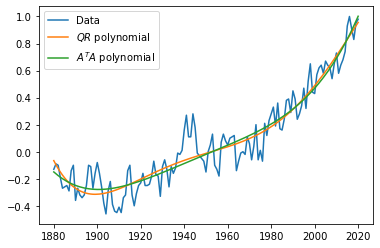
\includegraphics[width=100mm]{pr3_1.png}
		\caption{Dades i aproximacions polinomiques}
		\end{center}
	\end{figure}
	
	Podem veure que la $QR$ s'adapta una mica millor a la corba, i això es deu a que estem evitant treballar amb una matriu tan mal condicionada com es $A^TA$. Veiem pero que si escalem les dades, aleshores el nombre de condició de $A^TA$ disminueix fins a $cond(A^TA) = 1.3998\cdot 10^{7}$, extremadament millor que abans. Veiem ara que els polinomis en el interval $0$, $1$ se solapen.
	
	\begin{figure}[H]
		\begin{center}
		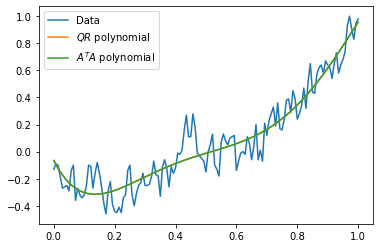
\includegraphics[width=100mm]{pr3_2.png}
		\caption{Dades i aproximacions polinomiques}
		\end{center}
	\end{figure}
	
\end{document}
